\section{Основные соотношения}

\begin{frame}
	\centering
	\Huge
	Математические модели
\end{frame}

\subsection{Основные соотношения}
\begin{frame}{Основные соотношения}
	Уравнения стационарной теплопроводности и равновесия в 2D
	\begin{gather*}
		\nabla \cdot \boldsymbol{q} = q_V,
		\quad
		-\nabla \cdot \widehat{\boldsymbol{\sigma}} = \boldsymbol{b}
	\end{gather*}
	где вектор плотности теплового потока $\boldsymbol{q}$ и тензор напряжений $\widehat{\boldsymbol{\sigma}}$ определены
	\begin{gather*}
		\boldsymbol{q}(\boldsymbol{x}) = 
			-p_1 \widehat{\boldsymbol{\lambda}} \cdot \nabla T
			-p_2 \int\limits_{S'(\boldsymbol{x}) \cap S} 
			    \varphi(|\boldsymbol{x} - \boldsymbol{x}'|) \widehat{\boldsymbol{\lambda}} \cdot \nabla T
			 dS'(\boldsymbol{x}), \\
		\widehat{\boldsymbol{\sigma}} =
		    p_1 \widehat{\text{\textbf{C}}} \cdot \cdot \left( \widehat{\boldsymbol{\varepsilon}} - \widehat{\boldsymbol{\alpha}}^T \Delta T \right) +
            p_2 \int\limits_{S'(\boldsymbol{x}) \cap S}
                \varphi(|\boldsymbol{x} - \boldsymbol{x}|) \widehat{\text{\textbf{C}}} \cdot \cdot \left( \widehat{\boldsymbol{\varepsilon}} - \widehat{\boldsymbol{\alpha}}^T \Delta T \right)
		    dS'(\boldsymbol{x}),
	\end{gather*}
	$p_1 > 0$ и $p_2 \geqslant 0$ --- весовые параметры модели, $p_1 + p_2 = 1$; \\
	$\varphi(|\boldsymbol{x} - \boldsymbol{x}'|)$~---~нормированная, положительная функция нелокального влияния, определённая на области $S'(\boldsymbol{x})$; \\
	$S'(\boldsymbol{x})$ --- область нелокального влияния с центром в точке $\boldsymbol{x} \in S$;\\
	$S$ --- область занимаемая рассматриваемым телом.
\end{frame}

\begin{frame}{Принятые гипотезы}
	Материал изотропный, а деформации малы, поэтому
	\begin{minipage}{0.62\textwidth}
		\begin{gather*}
		\widehat{\boldsymbol{\varepsilon}} = 
	\dfrac{\nabla \boldsymbol{u} + (\nabla \boldsymbol{u})^T}{2},
		\quad
		\widehat{\boldsymbol{\alpha}}^T = \alpha^T \widehat{\text{\textbf{I}}}_2,
		\quad
		\widehat{\boldsymbol{\lambda}} = \lambda \widehat{\text{\textbf{I}}}_2, \\
		C_{ijkl} =
		\dfrac{\nu E}{1 - \nu^2} \delta_{ij} \delta_{kl} +
		\dfrac{E}{2(1 + \nu)} (\delta_{ik} \delta_{jl} + \delta_{il} \delta_{jk}).
	\end{gather*}
	\end{minipage}
	\begin{minipage}{0.37\textwidth}
		\begin{center}
		\center{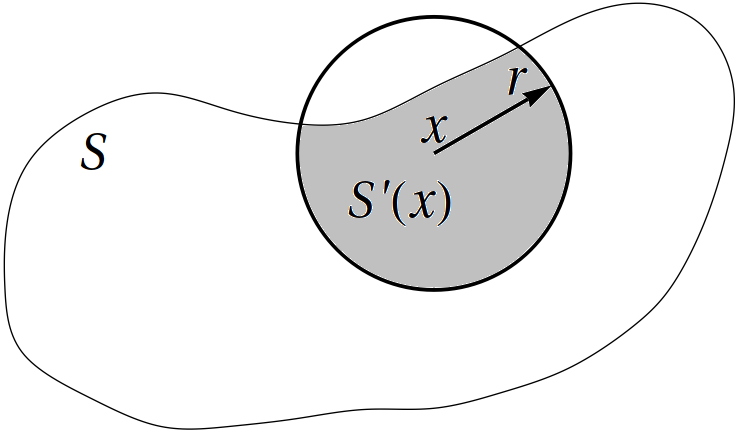
\includegraphics[width=\textwidth]{pics/NonlocalArea.png}} \\
		Область $S'(\boldsymbol{x})$, заданная радиусом~нелокальности~$r$.
	\end{center}
	\end{minipage}
	Граничные условия
	\begin{gather*}
		T|_{\Gamma_1} = T_{\Gamma} (\boldsymbol{x}),
		\quad
		\boldsymbol{n} \cdot \boldsymbol{q}|_{\Gamma_2} = f(\boldsymbol{x}),
		\quad
		\boldsymbol{n} \cdot \boldsymbol{q}|_{\Gamma_3} = \alpha (T_a(\boldsymbol{x}) - T(\boldsymbol{x}))), \\
		\boldsymbol{u}|_{\Gamma_4} = \boldsymbol{d} (\boldsymbol{x}),
		\quad
		\boldsymbol{n} \cdot \widehat{\boldsymbol{\sigma}}|_{\Gamma_5} = \boldsymbol{p} (\boldsymbol{x}).
	\end{gather*}
	
	
\end{frame}

\begin{comment}
\subsection{Нелокальный интегральный оператор}
\begin{frame}{Нелокальный интегральный оператор}
	\begin{gather*}
		\mathcal{N} [f(\boldsymbol{x})] = 
		p_1 f(\boldsymbol{x}) + 
		p_2 \int\limits_{S'(\boldsymbol{x}) \cap S} 
			\varphi(\boldsymbol{x}, \boldsymbol{x}') f(\boldsymbol{x}')
		dS'(\boldsymbol{x}),
		\quad
		\boldsymbol{x}' \in S'(\boldsymbol{x}).
	\end{gather*}
	$f(\boldsymbol{x})$ --- функция; $p_1 > 0$ и $p_2 \geqslant 0$ --- весовые параметры модели, $p_1 + p_2 = 1$; \\
	$\varphi(|\boldsymbol{x} - \boldsymbol{x}'|)$~---~нормированная, положительная функция нелокального влияния, определённая на области $S'(\boldsymbol{x})$; \\
	$S'(\boldsymbol{x})$ --- область нелокального влияния с центром в точке $\boldsymbol{x} \in S$;\\
	$S$ --- область занимаемая рассматриваемым телом.
	
	\begin{minipage}[b][][b]{0.32\linewidth}\centering
		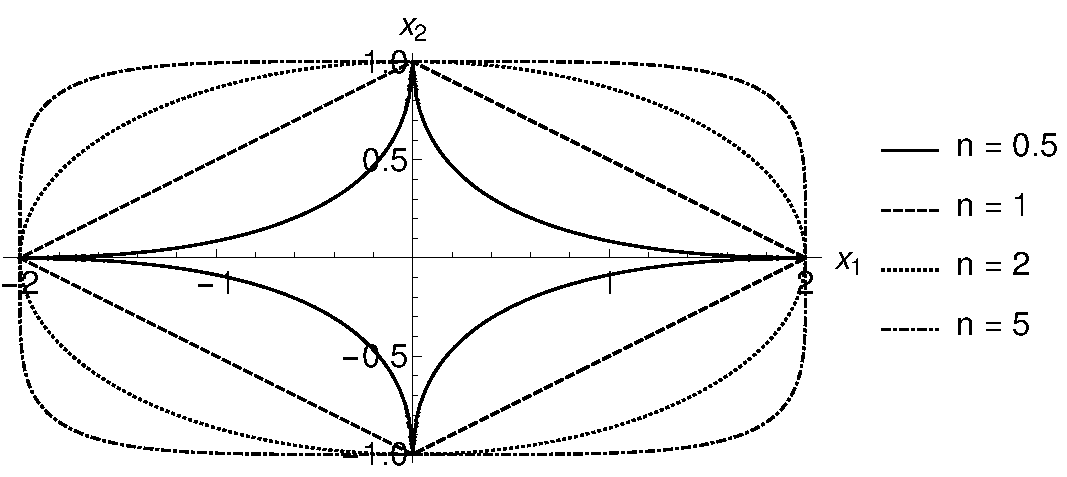
\includegraphics[width=\textwidth]{pics/SuperEllipse.pdf}
	\end{minipage}
    \hfill
    \begin{minipage}[b][][b]{0.32\linewidth}\centering
        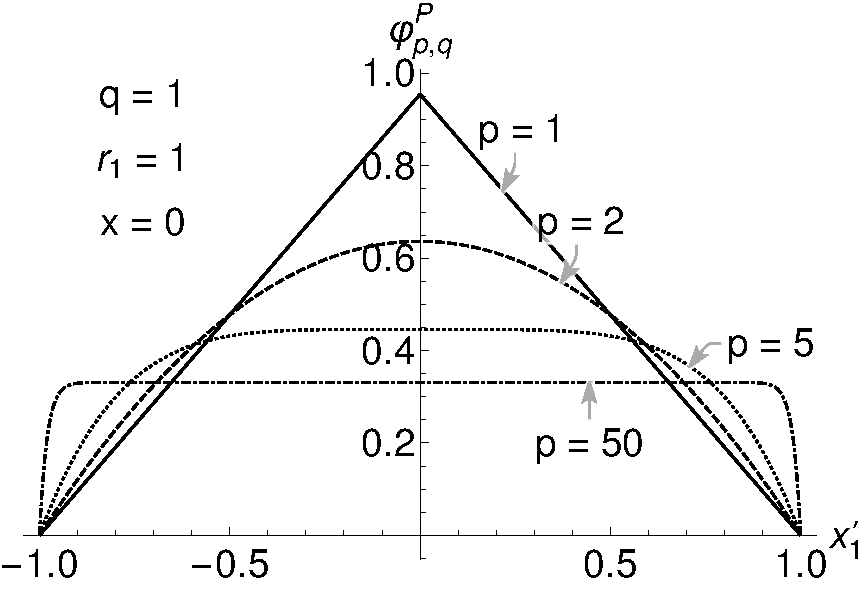
\includegraphics[width=\linewidth]{pics/PolynomialInfluenceP.pdf}
    \end{minipage}
    \hfill
    \begin{minipage}[b][][b]{0.32\linewidth}\centering
        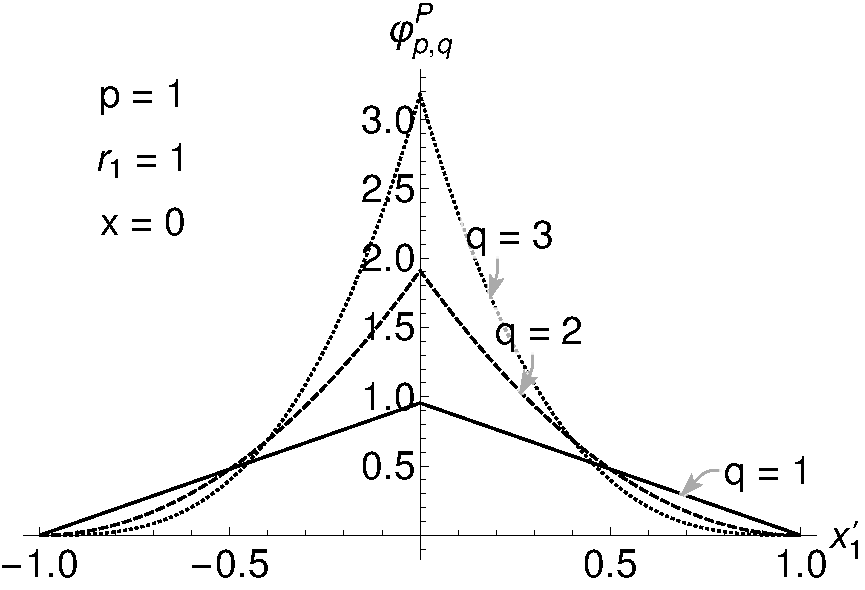
\includegraphics[width=\linewidth]{pics/PolynomialInfluenceQ.pdf}
    \end{minipage}
    \begin{center}
	    Возможные портреты функций влияния в сечении
    	\end{center}
\end{frame}

\subsection{Уравнения теплопроводности и равновесия}
\begin{frame}{Уравнения стационарной теплопроводности и равновесия}
	\begin{gather*}
		\nabla \cdot \boldsymbol{q} = q_V,
		\quad
		-\nabla \cdot \widehat{\boldsymbol{\sigma}} = \boldsymbol{b},
	\end{gather*}
	где вектор плотности теплового потока и тензор напряжений
	\begin{gather*}
		\boldsymbol{q}(\boldsymbol{x}) = 
			\mathcal{N} \left( -\widehat{\boldsymbol{\lambda}} \cdot \nabla T \right),
		\quad
		\widehat{\boldsymbol{\sigma}}(\boldsymbol{x}) =
		\mathcal{N} \left(
		\widehat{\text{\textbf{C}}} \cdot \cdot 
		\left( \widehat{\boldsymbol{\varepsilon}} - \widehat{\boldsymbol{\alpha}}^T \Delta T \right)
	\right).
	\end{gather*}
	Материал изотропный, а деформации малы, поэтому
	\begin{gather*}
		\widehat{\boldsymbol{\varepsilon}} = 
	\dfrac{\nabla \boldsymbol{u} + (\nabla \boldsymbol{u})^T}{2},
		\quad
		\widehat{\boldsymbol{\alpha}}^T = \alpha^T \widehat{\text{\textbf{I}}}_2,
		\quad
		\widehat{\boldsymbol{\lambda}} = \lambda \widehat{\text{\textbf{I}}}_2, \\
		C_{ijkl} =
		\dfrac{\nu E}{1 - \nu^2} \delta_{ij} \delta_{kl} +
		\dfrac{E}{2(1 + \nu)} (\delta_{ik} \delta_{jl} + \delta_{il} \delta_{jk}).
	\end{gather*}
	Граничные условия
	\begin{gather*}
		T|_{\Gamma_1} = T_{\Gamma} (\boldsymbol{x}),
		\quad
		\boldsymbol{n} \cdot \boldsymbol{q}|_{\Gamma_2} = f(\boldsymbol{x}),
		\quad
		\boldsymbol{n} \cdot \boldsymbol{q}|_{\Gamma_3} = \alpha (T_a(\boldsymbol{x}) - T(\boldsymbol{x}))), \\
		\boldsymbol{u}|_{\Gamma_4} = \boldsymbol{d} (\boldsymbol{x}),
		\quad
		\boldsymbol{n} \cdot \widehat{\boldsymbol{\sigma}}|_{\Gamma_5} = \boldsymbol{p} (\boldsymbol{x}).
	\end{gather*}
\end{frame}
\end{comment}

\section{Численный алгоритм решения}

\begin{frame}
	\centering
	\Huge
	Численный алгоритм решения
\end{frame}

\subsection{Матрично-векторные уравнения}
\begin{frame}{Конечно-элеметная аппроксимация уравнений}
	\justifying
	
	Матрично-векторные уравнения
	\begin{gather*}
		\left( p_1 \widehat{\textbf{K}}^L_T + p_2 \widehat{\textbf{K}}^{NL}_T + \widehat{\textbf{K}}^{\alpha}_T \right) \cdot \textbf{T} = \textbf{Q} + \textbf{F} + \textbf{T}^{\alpha}, \\
		\left( p_1 \widehat{\textbf{K}}^L_E + p_2 \widehat{\textbf{K}}^{NL}_E \right) \cdot \widehat{\textbf{U}} = \widehat{\textbf{B}} + p_1 \widehat{\textbf{E}}^L + p_2 \widehat{\textbf{E}}^{NL} + \widehat{\textbf{P}}.
	\end{gather*}
	
	Ассемблирование классических матриц
	\begin{gather*}
		\widehat{\textbf{K}}^L_{\mathcal{F}} =
		\color{blue}
		\sum\limits_{e \in S_h}
		\sum\limits_{n,m \in I^e}
		\color{red}
		\sum\limits_{q \in Q^e}
		\color{black}
		w_q \textbf{K}^{ee}_{nm} (\boldsymbol{x}_q, \boldsymbol{x}_q) J_q^e,
	\end{gather*}
	$\textbf{K}^{ee}_{nm}$ --- ядро интегрирование, зависящее от исследуемого \mbox{уравнения.}
	
	\color{blue} Синий \color{black} --- алгоритм, формирующий портрет матрицы.
	
	\color{red} Красный \color{black} --- интегрирование.
\end{frame}

\subsection{Аппроксимация интегрального слагаемого}
\begin{frame}{Аппроксимация интегрального слагаемого}
Квадратурная аппроксимация:
\begin{gather*}
	\footnotesize
	\widehat{\textbf{K}}^{NL}_T =
	\color{blue}
	\sum\limits_{e \in S_h}
	\sum\limits_{n \in I^{e}}
	\color{red}
	\sum\limits_{q \in Q^{e}}
	\color{black}
	w_q N_{n,i}^e(\boldsymbol{x}_q) J_q^{e} 
	\color{blue}
	\sum\limits_{e' \in S_h^{q}}
	\sum\limits_{m' \in I^{e'}}
	\color{red}
	\sum\limits_{q' \in Q^{e'}}
	\color{black}
	w_{q'} \varphi(\boldsymbol{x}_q, \boldsymbol{x}_{q'}) \lambda_{ij} N_{m',j}^{e'} (\boldsymbol{x}_{q'}) J_{q'}^{e'}.
\end{gather*}
Элементная аппроксимация:
\begin{gather*}
	\footnotesize
	\widehat{\textbf{K}}^{NL}_T =
	\color{blue}
	\sum\limits_{n \in S_h}
	\sum\limits_{e \in E^n}
	\sum\limits_{e' \in S_h^{e}}
	\sum\limits_{m' \in I^{e'}}
	\color{red}
	\sum\limits_{q \in Q^{e}} 
	\color{black}
	w_q N_{n,i}^e(\boldsymbol{x}_q) J_q^{e}
	\color{red}
	\sum\limits_{q' \in Q^{e'}}
	\color{black}
	w_{q'} \varphi(\boldsymbol{x}_q, \boldsymbol{x}_{q'}) \lambda_{ij} N_{m',j}^{e'} J_{q'}^{e'}.
\end{gather*}

\begin{minipage}[b][][b]{0.49\textwidth}
	\centering
	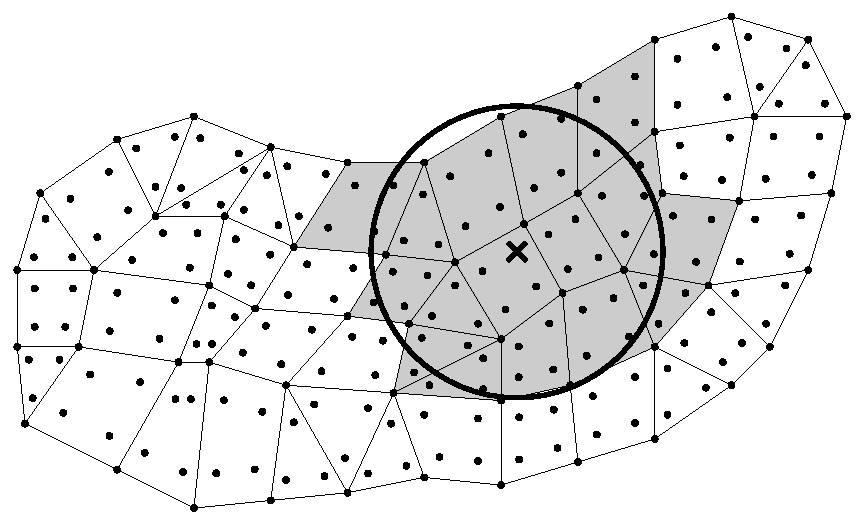
\includegraphics[width=\textwidth]{pics/ApproxSQ.pdf}
	Квадратурная аппроксимация
\end{minipage}
\hfill
\begin{minipage}[b][][b]{0.49\textwidth}
	\centering
	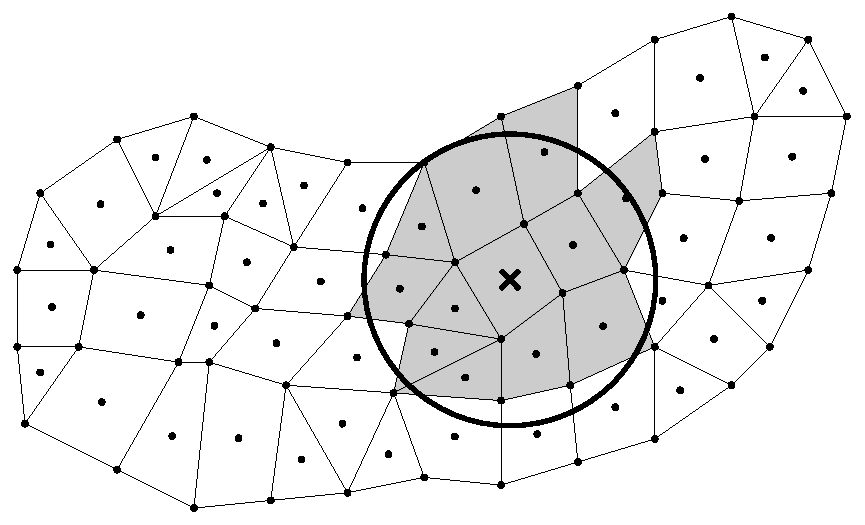
\includegraphics[width=\textwidth]{pics/ApproxSE.pdf}
	Элементная аппроксимация
\end{minipage}
\end{frame}

\section{Программный комплекс}

\begin{frame}
	\centering
	\Huge
	Программный комплекс NonLocFEM
\end{frame}

\subsection{Эффективность распараллеливания}
\begin{frame}{Эффективность распараллеливания}
	\begin{minipage}{0.49\textwidth}
		\centering
		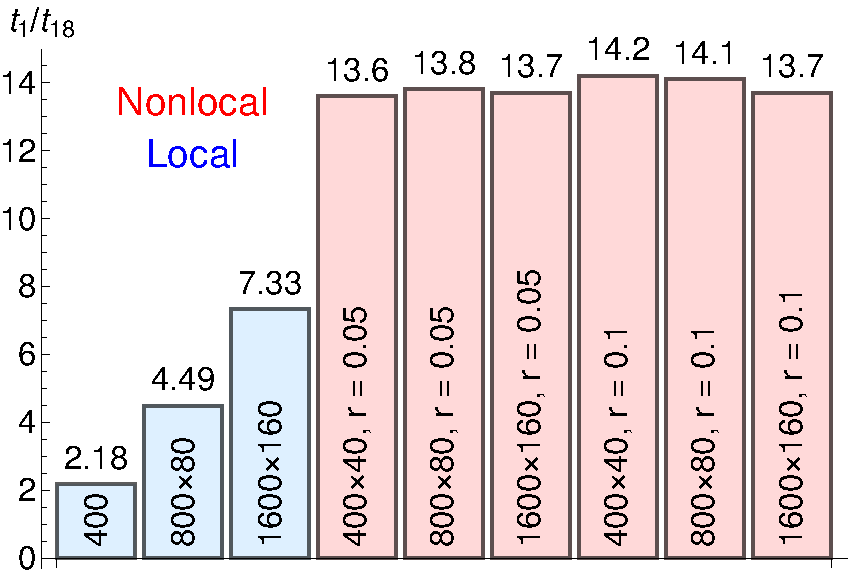
\includegraphics[width=0.75\textwidth]{pics/OMPThermalPresentation.pdf} \\
		Матрица теплопроводности
	\end{minipage}
	\begin{minipage}{0.49\textwidth}
		\centering
		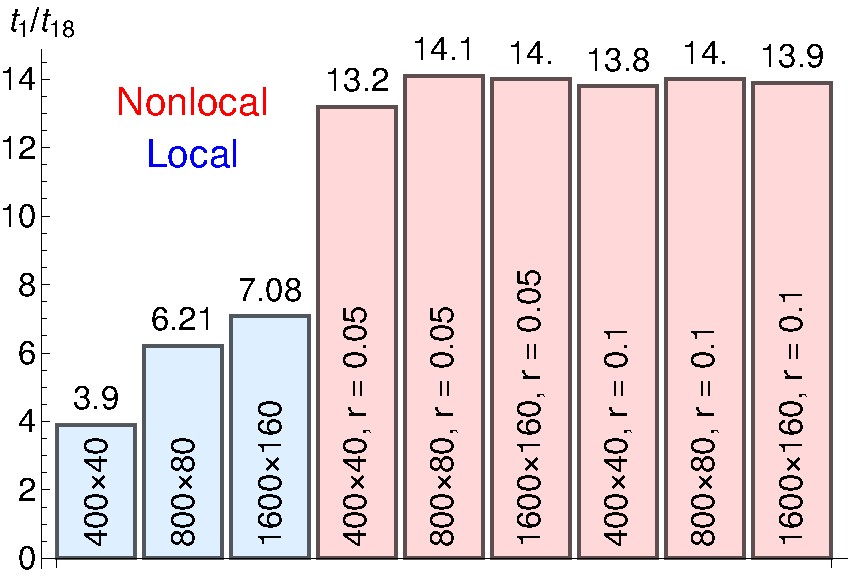
\includegraphics[width=0.75\textwidth]{pics/OMPMechanicalPresentation.pdf} \\
		Матрица жёсткости
	\end{minipage}
	\begin{center}
		Эффективность распараллеливания алгоритма сборки матриц
	\end{center}
	
\tiny
\begin{center}
	\centering
	\begin{tabular}{|c|c|c|c|c|c|}
	\hline
	Сетка & Радиус & \multicolumn{2}{c|}{Используемый объём}   & \multicolumn{2}{c|}{Время, с} \\
	      & поиска & \multicolumn{2}{c|}{оперативной памяти} & \multicolumn{2}{c|}{18 потоков} \\
	\hhline{~~----}
	      &        & $\widehat{\textbf{K}}_T$ & $\widehat{\textbf{K}}_E$ & $\widehat{\textbf{K}}_T$ & $\widehat{\textbf{K}}_E$ \\
	\hline
	$400 \times 40$   & 0    & 6.2 Мб  & 23.8 Мб  & 0.028 & 0.048 \\
	\hline
	$800 \times 80$   & 0    & 24.5 Мб & 95 Мб    & 0.116 & 0.274 \\
	\hline
	$1600 \times 160$ & 0    & 97.8 Мб & 379 Мб   & 0.705 & 2.366 \\
	\hline
	$400 \times 40$   & 0.05 & 61.4 Мб & 244 Мб   & 1.055 & 1.288 \\
	\hline
	$800 \times 80$   & 0.05 & 548 Мб  & 2.2 Гб   & 11.37 & 13.3  \\
	\hline
	$1600 \times 160$ & 0.05 & 5.5 Гб  & 22 Гб    & 132.9 & 155   \\
	\hline
	$400 \times 40$   & 0.1  & 133 Мб  & 532 Мб   & 2.68  & 3.26  \\
	\hline
	$800 \times 80$   & 0.1  & 1.34 Мб & 5.4 Гб   & 32    & 37.8  \\
	\hline
	$1600 \times 160$ & 0.1  & 17 Гб   & \textbf{68 Гб} & 447   & 521   \\
	\hline
	\end{tabular}
	
	\normalsize
	Занимаемая оперативная память и время ассемблирования матриц
\end{center}
\end{frame}


\subsection{Ускорение решения СЛАУ}
\begin{frame}{Ускорение решения СЛАУ}
	\justifying
	Существует несколько способов, которые могут повысить эффективность итерационных решателей СЛАУ:
	
	\begin{minipage}{0.49\textwidth}
		\begin{itemize}
			\item Оптимизация сетки
			\item Предобуславливатель
			\item Начальное приближение
			\item Оптимизация базиса элементов
		\end{itemize}
		
		Число обусловленности
		\begin{gather*}
			\text{cond} \widehat{\textbf{K}} = \sqrt{\dfrac{|\lambda_{\max}|}{|\lambda_{\min}|}}.
		\end{gather*}
	\end{minipage}
	\hfill
	\begin{minipage}{0.5\textwidth}
		\center{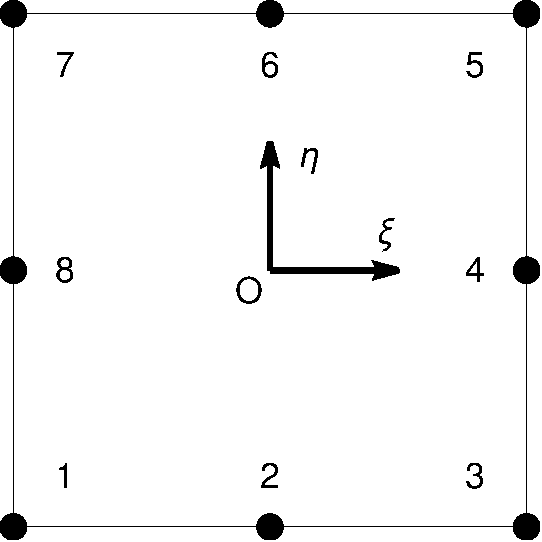
\includegraphics[width=0.65\textwidth]{pics/QuadraticSerendipity.pdf}}
		Квадратичный серендиповый элемент
	\end{minipage}
\end{frame}

\subsection{Параметрический базис элемента}
\begin{frame}{Параметрический базис элемента}
\begin{gather*}
    N_i = \dfrac{1}{16} (1 + \xi_i \xi) (1 + \eta_i \eta) ((9s - 1) (1 - \xi_i \xi - \eta_i \eta) + (9s + 3) \xi_i \xi \eta_i \eta), \\
    i = 1, 3, 5, 7; \xi_i, \eta_i = \pm 1, \\
    N_i = \dfrac{1}{16} (1 - \xi^2) (1 + \eta_i \eta) ((5 - 9s) + (9s + 3)\eta_i \eta),
    \quad
    i = 2, 6; \ \eta_i = \pm 1, \\
    N_i = \dfrac{1}{16} (1 - \eta^2) (1 + \xi_i \xi) ((5 - 9s) + (9s + 3)\xi_i \xi),
    \quad
    i = 4, 8; \ \xi_i = \pm 1.
\end{gather*}
Выбор параметра $s$ был основан на следующих предположениях
\begin{gather*}
    \int\limits_{-1}^{1} \int\limits_{-1}^{1} N_i (\xi, \eta) d\xi d\eta = s,
    \
    i = 1, 3, 5, 7, \quad
    \int\limits_{-1}^{1} \int\limits_{-1}^{1} N_i (\xi, \eta) d\xi d\eta = 1 - s,
    \
    i = 2, 4, 6, 8.
\end{gather*}
Классический базис получаем при \framebox{$s = -1 / 3$}.

Минимальный след матрицы оценим следующим образом
\begin{gather*}
	\label{eq:ParamSOptimal}
	\min\limits_s \int\limits_{-1}^{1} \int\limits_{-1}^{1} \sum\limits_{i = 0}^8 \sum\limits_{j = 0}^2 c_{j} N_{i, j}^2(\xi, \eta) d\xi d\eta =
	\min\limits_s C (27 s^2 -12 s + 19) \
	\rightarrow \ \text{\framebox{$s = \dfrac{2}{9}$}}.
\end{gather*}
\end{frame}

\subsection{Скорость сходимости решателя СЛАУ}
\begin{frame}{Скорость сходимости решателя СЛАУ}
Связь собственных чисел:
$\lambda_{\max}^{NL} = p_1 \lambda_{\max}^{L}$;
$\lambda_{\min}^{NL} \approx \lambda_{\min}^{L}$.

\begin{figure}[h]
	\begin{minipage}{0.49\textwidth}
		\centering
		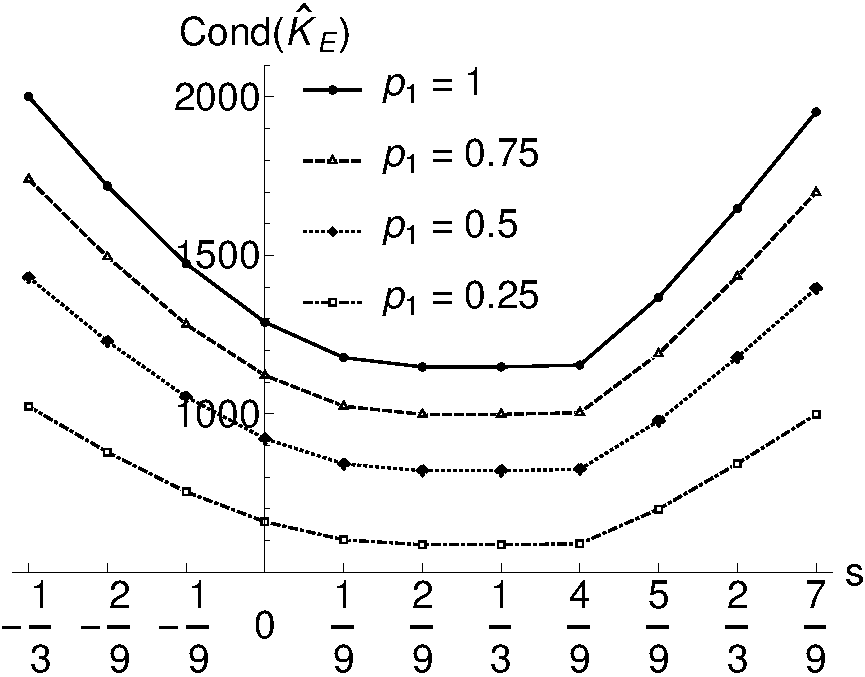
\includegraphics[width=0.7\textwidth]{pics/MechanicalCond.pdf} \\
		(а) число обусловленности
	\end{minipage}
	\begin{minipage}{0.5\textwidth}
		\centering
		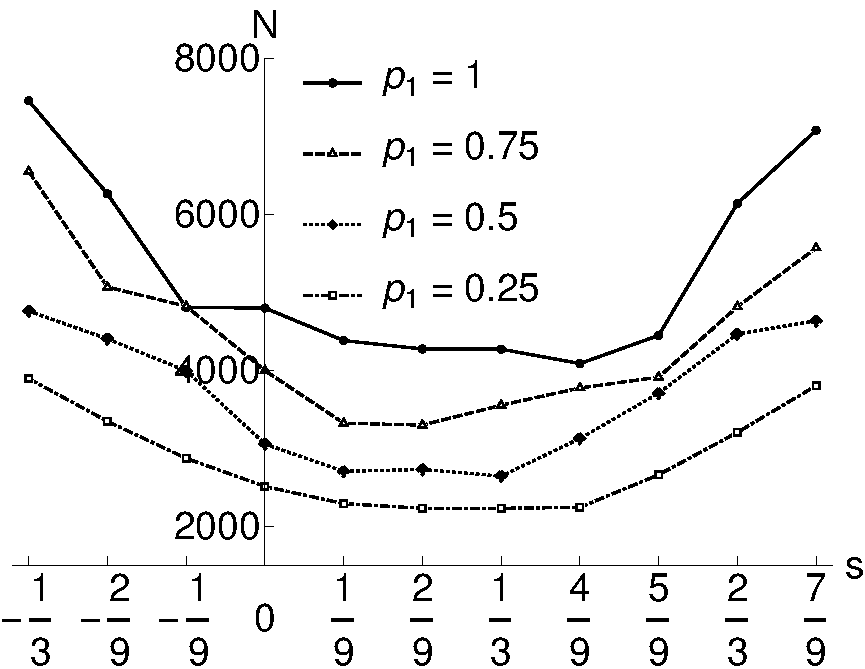
\includegraphics[width=0.7\textwidth]{pics/MechanicalIter.pdf} \\
		(б) количество итераций
	\end{minipage}
	\label{fig:ThermalCondAndIter}
\end{figure}

\begin{center}
\begin{tabular}{|c|c|c|c|}
	\hline
	$p_1$ & Id & ILLT$\left( \widehat{\textbf{K}}^L_E \right)$ & ILLT$\left( \widehat{\textbf{K}}^L_E \right)$ + $T_0$ \\
	\hline
	0.75 & 6330 & 2902 & 2736 \\
	0.5  & 5167 & 2290 & 2389 \\
	0.25 & 3779 & 1718 & 1740 \\
	\hline
\end{tabular}
\end{center}

Id --- единичный предобуславливатель;

ILLT$\left( \widehat{\textbf{K}}^L_E \right)$ --- неполное разложение Холецкого классической матрицы;

$T_0$ --- решение классической задачи при тех же граничных условиях.
\end{frame}

\subsection{Структура комплекса}
\begin{frame}{Структура программного комплекса NonLocFEM}
\begin{minipage}{0.49\textwidth}
	Возможные постановки:
	\begin{itemize}
		\justifying
		\footnotesize
		\item стационарная и нестационарная теплопроводность (1D, 2D);
		\item статические задачи несвязанной термоупругости (2D);
		\item граничные условия I, II, III родов и излучение;
		\item кинематические и силовые граничные условия;
		\item задачи идеального контакта с использование произвольного количества материалов;
		\item возможность использовать изотропные и ортотропные материалы.
	\end{itemize}
\end{minipage}
\hfill
\begin{minipage}{0.49\textwidth}
	\centering
	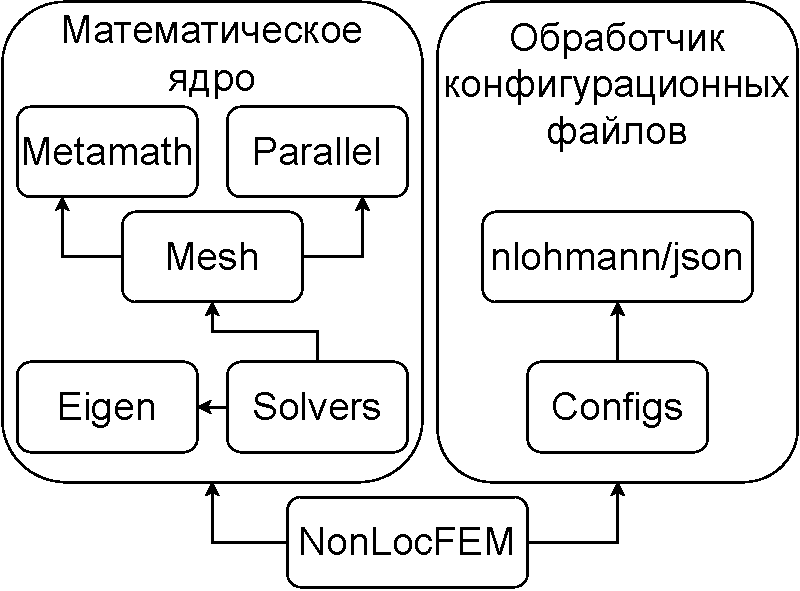
\includegraphics[width=\textwidth]{pics/NonLocFEMSchema.pdf}
	
	Структура программы NonLocFEM*
\end{minipage}
\bigskip

\justifying
* Свидетельство о государственной регистрации программы для ЭВМ \\
    №2021661966. NonLocFEM / А. А. Соколов, И. Ю. Савельева. Зарегистрировано в Реестре программ для ЭВМ 20.07.2021.
\end{frame}

\section{Анализ решений}

\begin{frame}
	\centering
	\Huge
	Анализ решений
\end{frame}

\subsection{Принципы Сен-Венана}
\begin{frame}{Принципы Сен-Венана и стабильности тепловых потоков}
\justifying
Область $S = [-5, 5] \times [-0.5, 0.5]$, сетка $S_h$ включает $1500 \times 150$ элементов.\\
Рассмотрим граничные, геометрические и интегральные условия
\begin{gather*}
	\boldsymbol{n} \cdot \overline{\boldsymbol{q}} |_{\overline{x}_1 = -5} = f(\overline{x}_2),
	\quad
	\boldsymbol{n} \cdot \overline{\boldsymbol{q}} |_{\overline{x}_1 = 5} = -f(\overline{x}_2),
	\quad
	\int\limits_S T dS = 0, \\
	\boldsymbol{n} \cdot \widehat{\boldsymbol{\sigma}} |_{x_1 = 0} = -f(x_2),
	\quad
	\boldsymbol{n} \cdot \widehat{\boldsymbol{\sigma}} |_{x_1 = 10} = f(x_2),
	\quad
	u_1 |_{x_1 = 0.5} = 0,
	\quad
	u_2 |_{x_2 = 5} = 0.
\end{gather*}
В качестве $f$ возьмём одно из трёх нагружений
\begin{gather*}
	f_1 (x) = 1,
	\quad
	f_2 (x) = 2 - 4 |x|,
	\quad
	f_3 (x) = 4 |x|,
\end{gather*}

\centering
\begin{minipage}{0.49\textwidth}
	\centering
	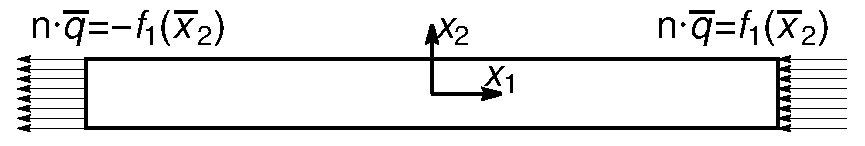
\includegraphics[width=\textwidth]{pics/RectangleFluxF1.pdf} \\
	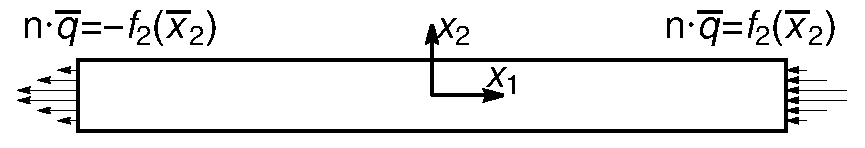
\includegraphics[width=\textwidth]{pics/RectangleFluxF2.pdf} \\
	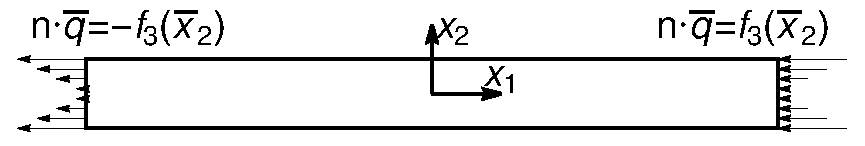
\includegraphics[width=\textwidth]{pics/RectangleFluxF3.pdf} \\
\end{minipage}
\begin{minipage}{0.49\textwidth}
	\centering
	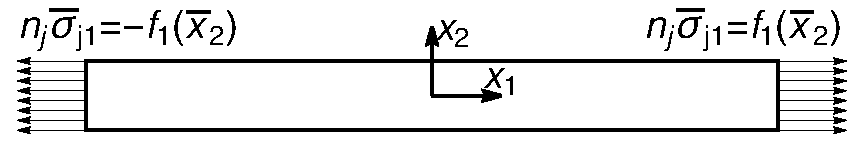
\includegraphics[width=\textwidth]{pics/RectangleStressF1.pdf} \\
	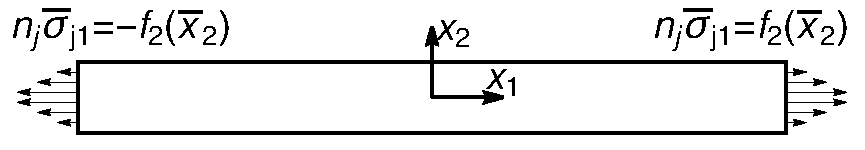
\includegraphics[width=\textwidth]{pics/RectangleStressF2.pdf} \\
	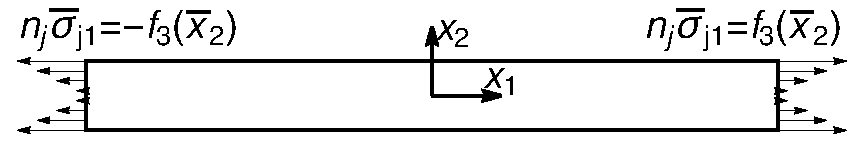
\includegraphics[width=\textwidth]{pics/RectangleStressF3.pdf} \\
\end{minipage}
Тепловые и механические нагружения, прикладываемые к пластине на левой и правой границах
\end{frame}


\begin{frame}
	\centering
	\begin{minipage}{0.4\textwidth}
		\centering
		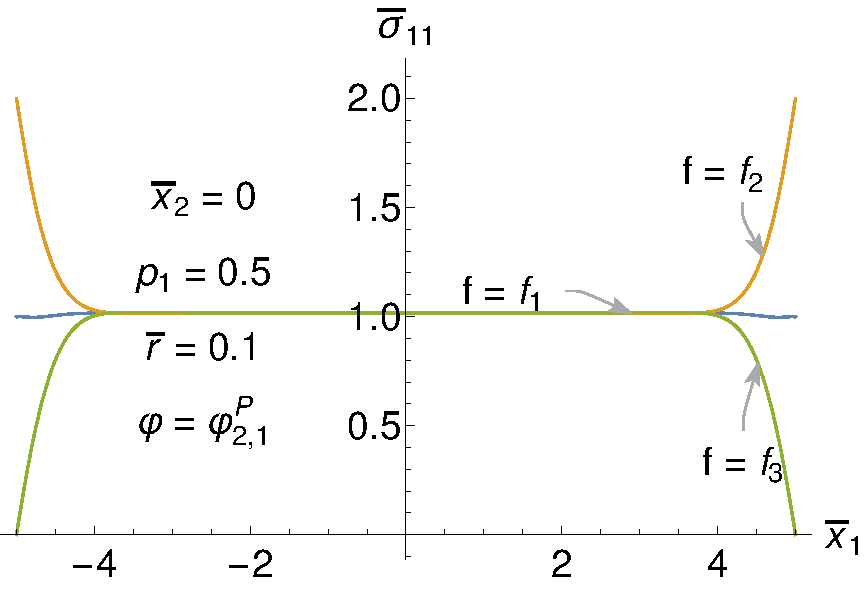
\includegraphics[width=\textwidth]{pics/SaintVenantX0P05Presentation.pdf} \\
		(а)
	\end{minipage}
	\begin{minipage}{0.4\textwidth}
		\centering
		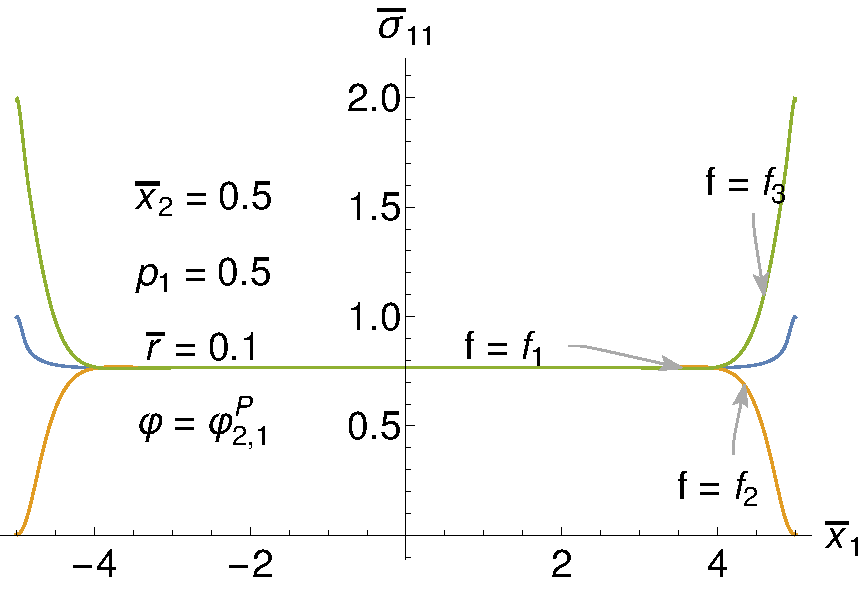
\includegraphics[width=\textwidth]{pics/SaintVenantX05P05Presentation.pdf} \\
		(б)
	\end{minipage}
	
	Распределения напряжения $\overline{\sigma}_{11}$ в сечениях вдоль оси нагружения
	
	\begin{minipage}{0.4\textwidth}
		\centering
		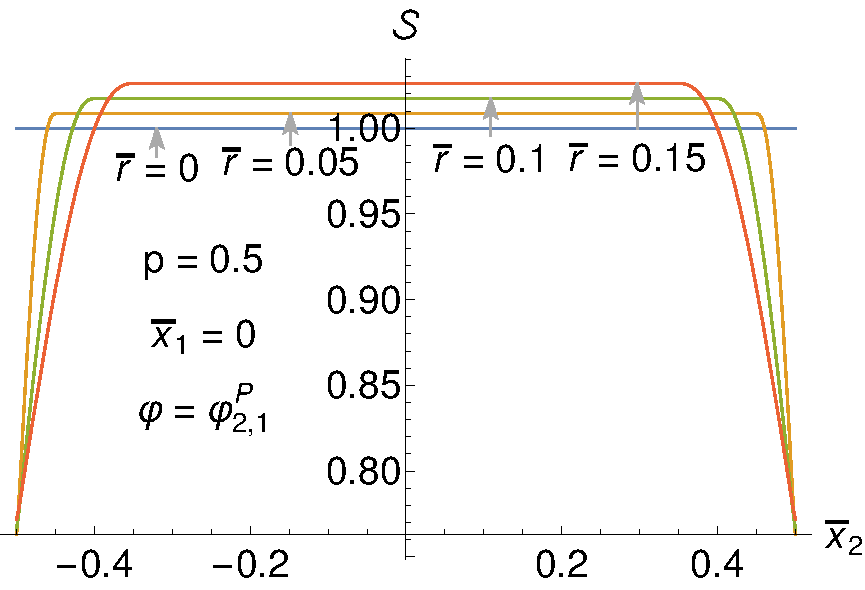
\includegraphics[width=\textwidth]{pics/HeatFluxStabilityVariationRPresentation.pdf} \\
		(а)
	\end{minipage}
	\begin{minipage}{0.4\textwidth}
		\centering
		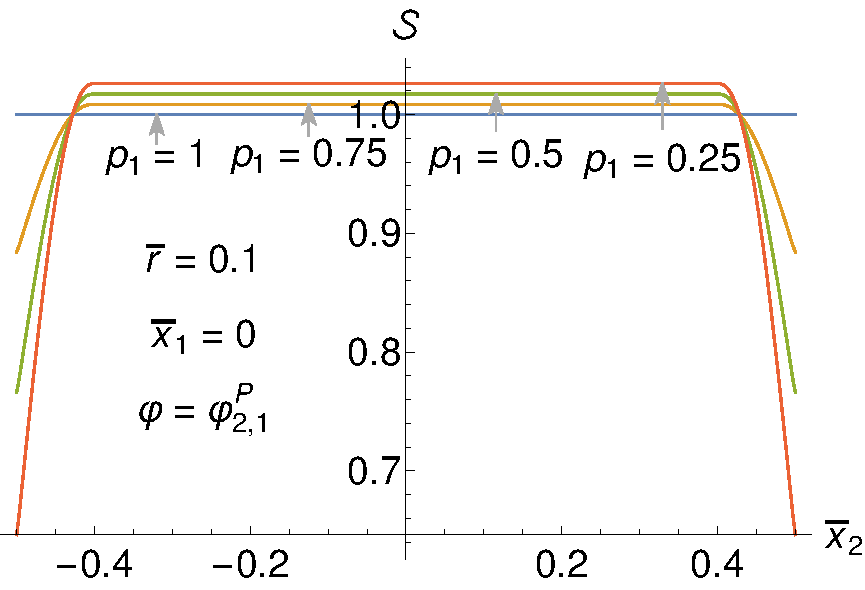
\includegraphics[width=\textwidth]{pics/HeatFluxStabilityVariationP1Presentation.pdf} \\
		(б)
	\end{minipage}
	
	Распределение напряжения $\overline{\sigma}_{11}$ в сечении поперёк оси нагружения
\end{frame}

\subsection{Задача Кирша}
\begin{frame}{Задача Кирша с обобщением на эллиптические вырезы}
Граничные и геометрические условия
\begin{gather*}
	n_j \overline{\sigma}_{j2} |_{x_1 = -1} = -1,
	\quad
	n_j \overline{\sigma}_{j2} |_{x_1 =  1} =  1,
	\quad
	u_1 |_{x_2 = 0} = 0,
	\quad
	u_2 |_{x_1 = 0} = 0.
\end{gather*}
\begin{minipage}{0.49\textwidth}
	Координаты на дуге AB
	\begin{gather*}
		\begin{cases}
			x_1 (\theta) = R_1 \cos \theta, \\
			x_2 (\theta) = R_2 \sin \theta.
		\end{cases}
	\end{gather*}
	Натуральный параметр длины
\begin{gather*}
	l (\theta) = \int\limits_0^{\theta} \sqrt{
		\left( \dfrac{\partial x_1}{\partial \varphi} \right)^2 +
		\left( \dfrac{\partial x_2}{\partial \varphi} \right)^2
	} d \varphi.
\end{gather*}
Обезразмерим параметр длины
\begin{gather*}
	\overline{l} (\theta) = \dfrac{l (\theta)}{l \left( \dfrac{\pi}{2} \right)},
	\quad
	0 \leqslant \theta \leqslant \dfrac{\pi}{2}.
\end{gather*}
\end{minipage}
\begin{minipage}{0.49\textwidth}
	\justifying
	Область $S \subset [-1, 1] \times [-1, 1]$, сетка $S_h$, где $h \approx 0.005$.
	\begin{center}
		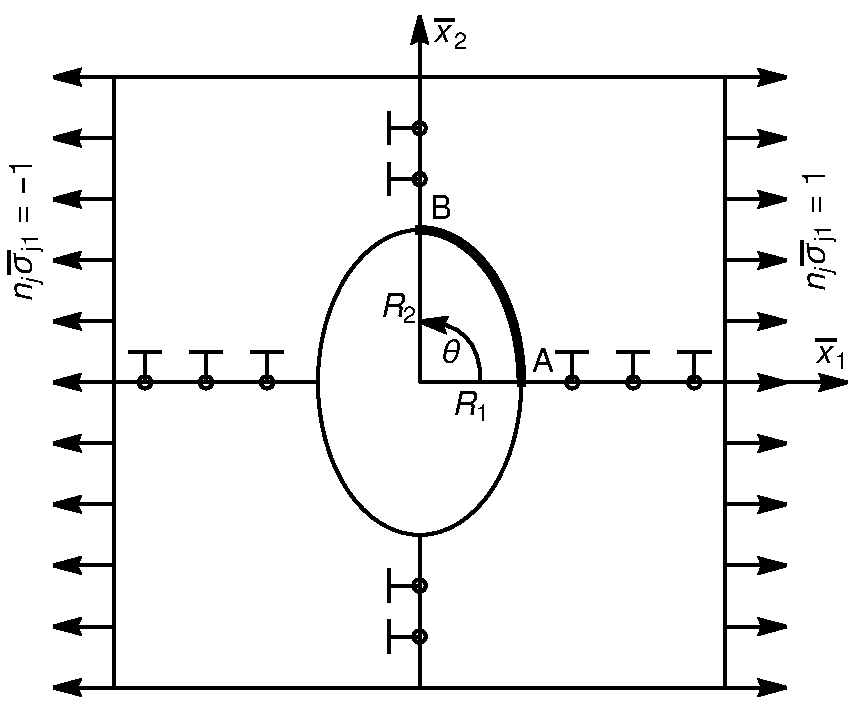
\includegraphics[width=0.9\textwidth]{pics/EllipseStressPresentation.pdf}
		Область с эллиптическим вырезом
	\end{center}
\end{minipage}
\end{frame}


\begin{frame}
\begin{minipage}{0.59\textwidth}
	Отношение длин полуосей
	\begin{gather*}
		\rho = R_2 / R_1.
	\end{gather*}
	Максимальные напряжения
	\begin{gather*}
		\overline{\sigma}_{11}^{\max} = \kappa (p_1) \left( 1 + 2 \rho \right) \sigma_0.
	\end{gather*}	
	Множитель зависящий от $p_1$
	\begin{gather*}
		\kappa (p_1) = \dfrac{1}{n} \sum\limits_{i = 0}^{n} \dfrac{\overline{\sigma}_{11}^{\max} (\rho_i, p_1)}{\overline{\sigma}_{11}^{\max} (\rho_i, 1)}.
	\end{gather*}

	\tiny
	\centering
	\begin{tabular}{|c|c|c|c|c|}
		\hline
		          $\rho$  & \multicolumn{4}{c|}{Весовые параметры} \\
		\cline{2-5}
		                  & $p_1 = 1$ & $p_1 = 0.75$ & $p_1 = 0.5$ & $p_1 = 0.25$ \\
		\hline
		$0.5$             & 2.012     & 1.783        & 1.537       & 1.510 \\
		\hline
		$0.75$            & 2.578     & 2.235        & 1.919       & 1.727 \\
		\hline
		$1$               & \textbf{3.053} & 2.696        & 2.308       & 1.937 \\
		\hline
		$1.25$            & 3.532     & 3.123        & 2.670       & 2.139 \\
		\hline
		$1.5$             & 4.012     & 3.551        & 3.031       & 2.404 \\
		\hline
		$\kappa$ & 1         & 0.881        & 0.755       & 0.652 \\
		\hline
	\end{tabular}
	Максимальный уровень напряжения $\overline{\sigma}_{11}$ при вариации отношения длин полуосей $\rho$ и весового параметра $p_1$, где $\overline{r} = 0.05$
\end{minipage}
\begin{minipage}{0.39\textwidth}
	\centering
	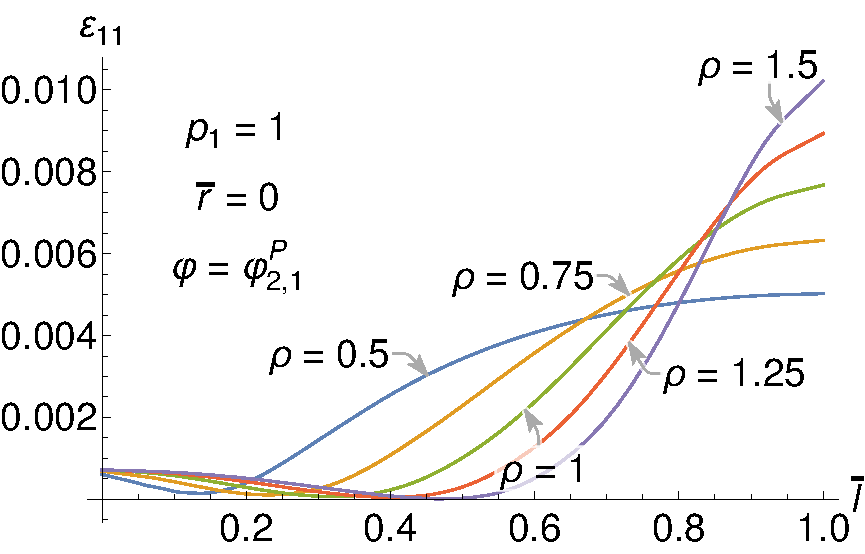
\includegraphics[width=\textwidth]{pics/KirshABEps11LocalPresentation.pdf} \\
	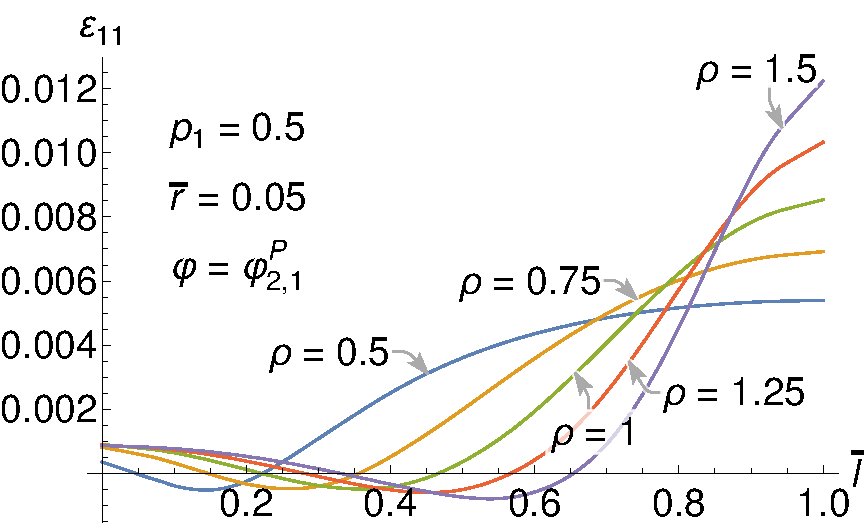
\includegraphics[width=\textwidth]{pics/KirshABEps11r005p05Presentation.pdf} \\
	
	Распределение деформации в локальном и нелокальном случаях
\end{minipage}
\end{frame}


\subsection{Температурные деформации}
\begin{frame}{Температурные деформации на области с вырезом}
	Рассмотрим ту же область, что была на задаче Кирша, но поставим тепловое нагружение на границах
\begin{gather*}
	\boldsymbol{n} \cdot \overline{\boldsymbol{q}}|_{\overline{x}_1 = -1} = 1,
	\quad
	\boldsymbol{n} \cdot \overline{\boldsymbol{q}}|_{\overline{x}_1 = 1} = -1,
	\quad
	\overline{u}_2 |_{\overline{x}_1 = 0} = 0.
\end{gather*}
\begin{minipage}{0.49\textwidth}
	Для единственности решения поставим интегральные условия на температуру и первую компоненту перемещения
	\begin{gather*}
		\int\limits_S \overline{T} dS = 0,
		\quad
		\int\limits_S \overline{u}_1 dS = 0.
	\end{gather*}
\end{minipage}
\begin{minipage}{0.49\textwidth}
	\centering
	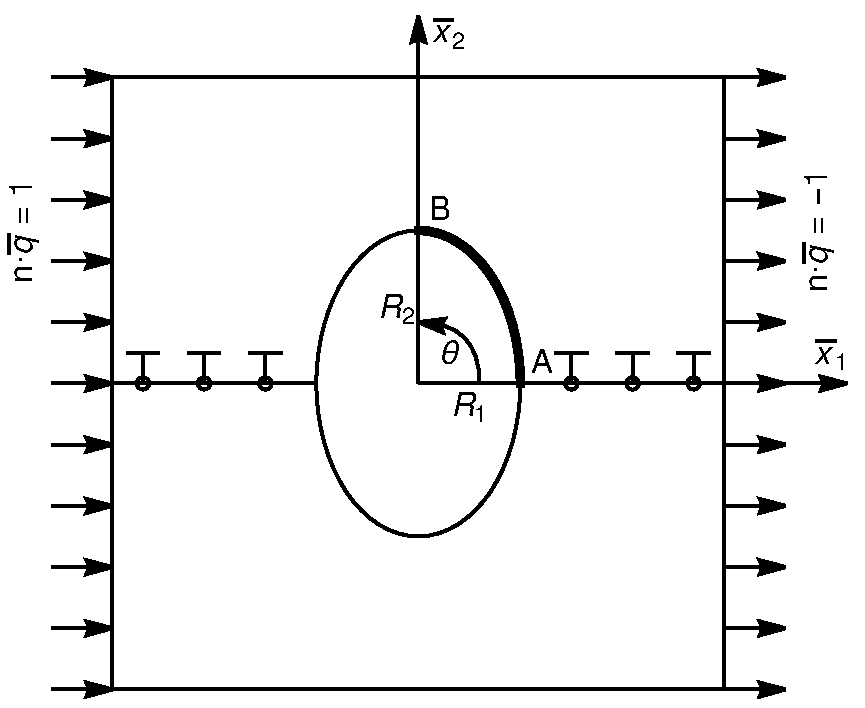
\includegraphics[width=0.8\textwidth]{pics/EllipseThermalPresentation.pdf}
	Область с эллиптическим вырезом и тепловыми граничными условиями
\end{minipage}
\end{frame}


\begin{frame}
\centering
\begin{minipage}{0.45\textwidth}
	\centering
	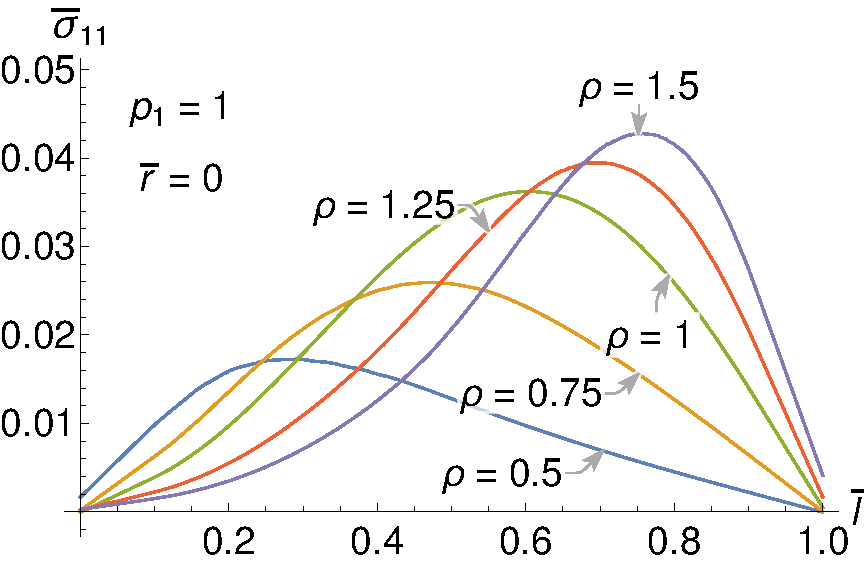
\includegraphics[width=\textwidth]{pics/ThermalKirshSigma11LocalPresentation.pdf} \\
\end{minipage}
\begin{minipage}{0.45\textwidth}
	\centering
	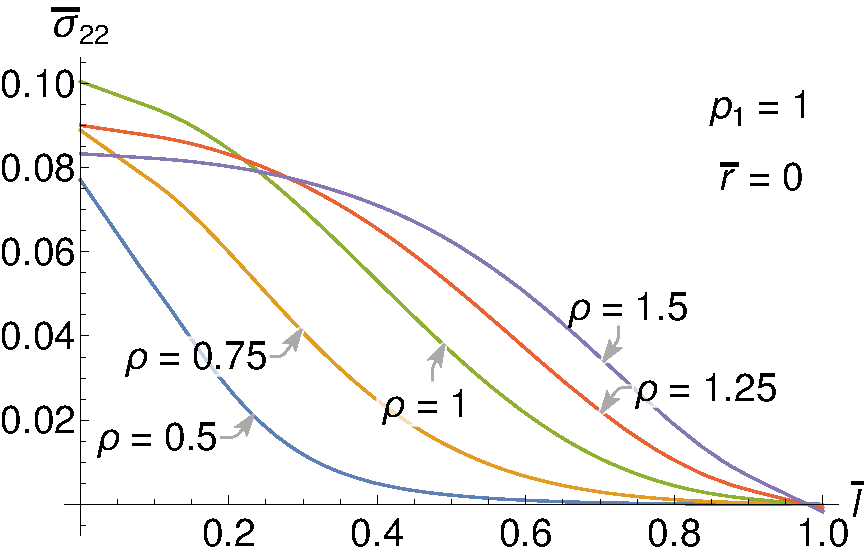
\includegraphics[width=\textwidth]{pics/ThermalKirshSigma22LocalPresentation.pdf} \\
\end{minipage}

Распределение напряжений $\overline{\sigma}_{11}$ и $\overline{\sigma}_{22}$ при вариации соотношения $\rho$

\bigskip
\bigskip

\begin{minipage}{0.45\textwidth}
	\centering
	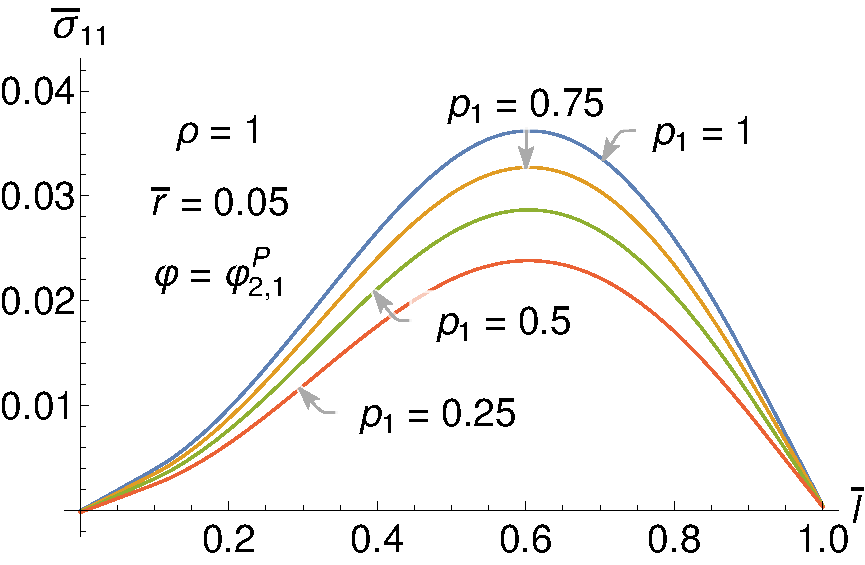
\includegraphics[width=\textwidth]{pics/ThermalKirshSigma11VariationP1Presentation.pdf} \\
\end{minipage}
\begin{minipage}{0.45\textwidth}
	\centering
	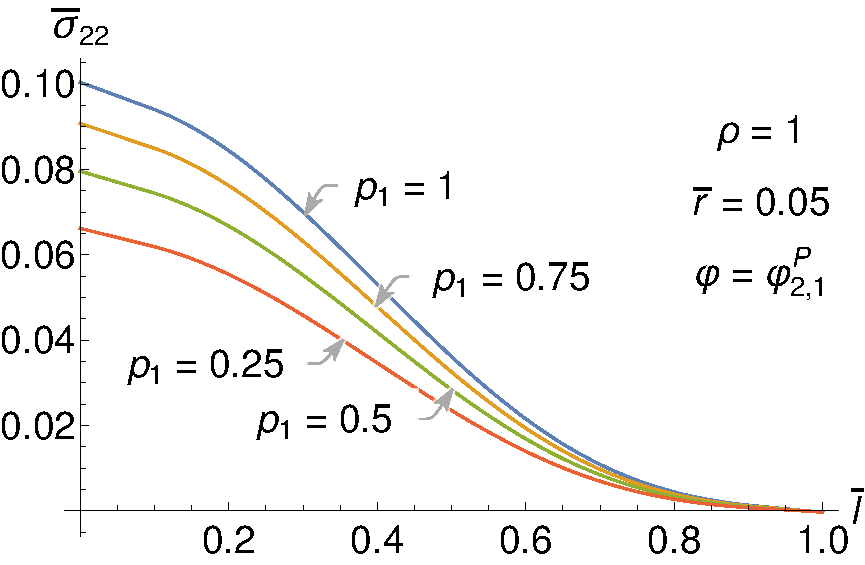
\includegraphics[width=\textwidth]{pics/ThermalKirshSigma22VariationP1Presentation.pdf} \\
\end{minipage}

Распределение напряжений $\overline{\sigma}_{11}$ и $\overline{\sigma}_{22}$ при вариации параметра $p_1$
\end{frame}